\documentclass[a4paper,12pt,onside]{report}
\usepackage[utf8]{inputenc}
\usepackage{a4wide,url}   
\usepackage{amsmath}  
\usepackage{amsfonts}
\usepackage{amssymb}
\usepackage{amsthm} 
\usepackage[french]{babel}
\usepackage{bbold}
\usepackage{bbm}
\usepackage{calligra}
\usepackage{color}
\usepackage{dsfont}
\usepackage{fancyhdr}
\usepackage[Glenn]{ fncychap}
\usepackage[T1]{fontenc}
\usepackage[left=3.5cm,right=3.5cm,top=3.5cm,bottom=3.5cm]{geometry}
\usepackage{graphics,graphicx,subfigure,wrapfig,picinpar}
\usepackage{lipsum}
\usepackage{lmodern}
\usepackage{microtype}
\usepackage{xspace}
\usepackage{xcolor}
\usepackage{wasysym}
\usepackage{fancyhdr}
\usepackage{epstopdf}
\usepackage{datetime}
\usepackage{hyperref}
\usepackage[all,cmtip]{xy}
\usepackage{listings}
\usepackage{caption}
\usepackage{pdfpages}
\usepackage{mathpazo} % use palatino
\usepackage[scaled]{helvet} % helvetica

\newtheorem {theorem}{Théorème}[chapter]
\newtheorem {lemme}{Lemme}[chapter]
\newtheorem {corollary}{Corollaire}[chapter]
\newtheorem {proposition}{Proposition}[chapter]
\newtheorem {definition}{Définition}[chapter]
\newtheorem*{ proof }{Preuve}
\newtheorem{remark}{Remarque}[chapter]


\newenvironment{prof}[1][Preuve]{\textbf{#1.} }{\ \rule{0.5em}{0.5em}}
%\theoremstyle{plain}
%\newtheorem{lemma}{Lemma}[chapter]
%\newtheorem{Propri\'et\'e}{Propri\'et\'e}[chapter]
\newtheorem{exercise}{Exercice}[chapter]
%\newtheorem{proposition}{Proposition}[chapter]
%\newtheorem{theorem}{Th\'eor\`eme}[chapter]
%\newtheorem{definition}{D\'efinition}[chapter]
\newtheorem{coro}{Corollaire}[chapter]
%\newtheorem{not}{Notation}[chapter]
\newtheorem{ex}{Exemple}[chapter]
%\newtheorem{property}{Propri\'et\'e}[section]
\newtheorem{theodef}{Th\'eor\`eme et D\'efinition}[chapter]
\newtheorem{rap}{Rappel}[chapter]
\newtheorem{thm}{Théoréme}[chapter]
\newtheorem{prop}{Proposition}[chapter]
\newtheorem{pro}{Propriétés}[chapter]
\newtheorem{lem}{lemme}[chapter]
\newtheorem{dfn}{Définition}[chapter]

\newtheorem{Post}{Postulat}



\DeclareGraphicsRule{.tif}{png}{.png}{`convert #1 `dirname #1`/`basename #1 .tif`.png}



\usepackage{eucal} 
\addtolength{\hoffset}{-1.0cm} 
\addtolength{\textwidth}{2.0cm}%1.6avant
\addtolength{\voffset}{-1.0cm} 
\addtolength{\textheight}{2.0cm}


\makeatletter
\newcommand{\thechapterwords}
{ \ifcase \thechapter\or Premier\or Deux\or Trois\or Quatre\or
Cinq\or
Six\or Sept\or Huit\or Neuf\or Dix\or Onze\fi}
\def\thickhrulefill{\leavevmode \leaders \hrule height 1ex \hfill \kern \z@}
\def\@makechapterhead#1{
\vspace*{15\p@}
{\parindent \z@ \centering \reset@font
\thickhrulefill\quad
\scshape \@chapapp{} \thechapterwords
\quad \thickhrulefill
\par\nobreak
\vspace*{15\p@}
\interlinepenalty\@M
\hrule
\vspace*{15\p@}
\Huge \bfseries #1\par\nobreak
\par
\vspace*{15\p@}
\hrule
\vskip 60\p@
}}
\def\@makeschapterhead#1{
\vspace*{15\p@}
{\parindent \z@ \centering \reset@font
\thickhrulefill
\par\nobreak
\vspace*{15\p@}
\interlinepenalty\@M
\hrule
\vspace*{15\p@}
\Huge \bfseries #1\par\nobreak
\par
\vspace*{15\p@}
\hrule
\vskip 60\p@
}}
\def\@makechapterhead#1{
\vspace*{15\p@}
{\parindent \z@ \centering \reset@font
\thickhrulefill\quad
\scshape \@chapapp{} \thechapterwords
\quad \thickhrulefill
\par\nobreak
\vspace*{15\p@}
\interlinepenalty\@M
\hrule
\vspace*{15\p@}
\Huge \bfseries #1\par\nobreak
\par
\vspace*{15\p@}
\hrule
\vskip 60\p@
}}
\frenchspacing \pagestyle{headings}
\usepackage{fancyhdr}
\pagestyle{fancy}

\usepackage [dvips]{epsfig}

\renewcommand{\sectionmark}[1]{\markboth{#1}{}}
\renewcommand{\sectionmark}[1]{\markright{\thechapter\ #1}}


\renewcommand{\sectionmark}[1]{\markboth{#1}{}}

\fancyhf{}

\fancyhead[L,R]{\bfseries\thepage}

\fancyhead[L]{\bfseries\rightmark} % Left Odd
\fancyhead[R]{\bfseries\leftmark} % Right Even
\renewcommand{\headrulewidth}{1pt}

\addtolength{\headheight}{1pt} 

\renewcommand{\footrulewidth}{0.5pt}

\fancypagestyle{plain}{ % pages de tetes de chapitre
\fancyhead{} % supprime l'entete
%\fancyfoot{} %supprime le pied de page
\renewcommand{\headrulewidth}{0pt}
}
\newcommand{\clearemptydoublepage}{%
\newpage{\pagestyle{plain}\cleardoublepage}}

\rhead{\textbf{\thepage}}
\lhead{\textsl{\leftmark}}
\fancyfoot[LO]{\tiny \emph{\textbf{Schémas monotones discrétisés en temps pour l'équation de Schrödinger}}} 

\usepackage{newlfont}

%\usepackage[active]{srcltx}
\hfuzz2pt
\newlength{\defbaselineskip}
\setlength{\defbaselineskip}{\baselineskip}
\newcommand{\setlinespacing}[1]%
{\setlength{\baselineskip}{#1 \defbaselineskip}}
\newcommand{\doublespacing}{\setlength{\baselineskip}%
{1.5 \defbaselineskip}}
\newcommand{\singlespacing}{\setlength{\baselineskip}{\defbaselineskip}}


\newcommand{\Z}{\mathbb Z}
\newcommand{\R}{\mathbb R}
\newcommand{\C}{\mathbb C}
\newcommand{\N}{\mathbb N}
\newcommand{\F}{\mathbb F}
%\newcommand{\1}{1 \! \! {\rm I}}
\newcommand{\cc}{\mathcal{C}}
\newcommand{\A}{\mathcal{A}}
\newcommand{\X}{\mathcal{X}}
\newcommand{\I}{\mathcal{I}}
\newcommand{\el}{\mathcal{L}}
\newcommand{\G}{\mathcal{G}}
\newcommand{\B}{\mathcal{B}}
\newcommand{\f}{\mathcal{F}}
\newcommand{\E}{\mathcal{E}}
%\newcommand{\H}{\mathcal{H}}
\newcommand{\M}{\mathcal{M}}
\newcommand{\W}{\mathcal{W}}
\newcommand{\n}{\mathcal{N}}
\newcommand{\ho}{\hbox{\rm Hom}}
\newcommand{\Q}{l \! \! \! Q}
\newcommand{\0}{/ \! \! \! 0}
%\newcommand{\a}{\mathcal{a}}
\newcommand{\g}{\mathfrak g}
\newcommand{\h}{\mathfrak h}
%\newcommand{\e}{\mathfrak e}
%\newcommand{\u}{\mathfrak u}

\usepackage{amssymb,textcomp}

\def\card{{\rm card }}

\usepackage{stmaryrd}
\begin{document}
\begin{titlepage}
\begin{center}

\begin{center}
\textsc{Memoire de Master}\\
\vspace{0.5cm}
\textsc{Filière: Mathématiques Fondamentales}\\
\vspace{1.2cm}
\textsc{\underline{Thème}}\\
\vspace{0.8cm}
\end{center}

\rule{\linewidth}{1mm}\\
\begin{center}
\textsc{\textbf{ \color{blue}{Schémas monotones discrétisés en temps pour l'équation de Schrödinger}}}
\end{center}
\rule{\linewidth}{1mm}
\vspace{1cm}
\begin{flushright}
\textbf{Présenté par:}\\
\vspace{0.2cm}
\textcolor{magenta}{Kenneth ASSOGBA}\\
\textcolor{black}{kennethassogba@gmail.com}\\
\vspace{1cm}
\textbf{\textcolor{black}Sous la direction de :}\\
\vspace{0.2cm}
\textcolor{magenta}{\textbf{Prof.} Julien SALOMON}\\
\textsc{Université Paris-Dauphine}\\
\vspace{0.2cm}
\end{flushright}
\vspace{2cm}
%\begin{flushleft}
%\textbf{Soutenu le 29 Novembre 2018 devant le jury composé de:}\\
%\vspace{0.5cm}
%$
%\begin{array}{ll}
%\mbox{Président du jury:}&\textbf{Prof. Aboubacar %MARCOS}\\\\
%\mbox{Membres du jury:}&\textbf{Prof. Guy DEGLA}\\\\
%&\textbf{Prof. Liamidi A. LEADI}
%\end{array}
%$
%\end{flushleft}
s
\vspace{4cm}
\begin{center}
\noindent \textbf{Année Universitaire : 2018-2019}
\end{center}
%\vspace{1cm}
%\rule{\linewidth}{1mm}
\end{center}
\end{titlepage}
%\newpage
%\bibliographystyle{plain}
\pagenumbering{roman}
%\input{Dedicace.tex}
%\input{Remerciements.tex}
\chapter*{Résumé \& Abstract}\addcontentsline{toc}{chapter}{Résumé \& Abstract}
\Large
\begin{flushleft}
\textbf{\underline{Résumé}}
\end{flushleft}
\normalsize
Les problèmes de contrôle optimal dans les systèmes quantiques suscitent un vif intérêt, aussi bien pour les questions fondamentales que pour les applications existantes et futures. Un problème important est le développement de méthodes de construction de contrôles pour les systèmes quantiques. Une des méthodes couramment utilisée est la méthode de Krotov initialement proposée dans un cadre plus général dans les articles de V.F. Krotov et I.N. Feldman (1978 \cite{Krotov1}, 1983 \cite{Krotov2}). Cette méthode a été utilisée pour développer une nouvelle approche permettant de determiner des contrôles optimaux pour les systèmes quantiques dans \cite{Tannor} et dans de nombreux autres travaux de recherche: \cite{Zhu}, \cite{Maday} et \cite{Salomon} notamment. Leur mise en œuvre numérique repose sur des discrétisations liées à des développement limités. Cette approche entraîne cependant parfois des instabilités numériques. Nous presentons ici plusieurs méthodes de discrétisation temporelle qui permettent de résoudre ce problème en conservant au niveau discret la monotonie des schémas.\\\\
\Large\textbf{\underline{Mots-clés}}\normalsize\\\\
contrôle quantique, schémas monotones convergents, methode de Krotov
\[\]
\Large\textbf{\underline{Abstract}}\\\\\normalsize
Mathematical problems of optimal control in quantum systems attract high interest in connection with fundamental questions and existing and prospective applications. An important problem is the development of methods for constructing controls for quantum systems. One of the commonly used methods is the Krotov method initially proposed beyond quantum control in the articles by V.F. Krotov and I.N. Feldman (1978 \cite{Krotov1}, 1983 \cite{Krotov2}). The method was used to develop a novel approach for finding optimal controls for quantum systems in \cite{Tannor}, and in many works of various scientists: \cite{Zhu}, \cite{Maday} et \cite{Salomon} especially. However, the properties of the discrete version of these procedures have not been yet tackled with.
We present here a stable time and space discretization which preserves the
monotonic properties of the monotonic algorithms.\\\\
\Large\textbf{\underline{Key words}}\normalsize\\\\
quantum control, monotonically convergent algorithms, Krotov method,

\chapter*{Notations}\addcontentsline{toc}{chapter}{Notations}
$
\begin{array}{ll}
\Omega & \mbox{Espace des configurations}\\\\
\mathcal{H} & \mbox{Espace de Hilbert correspondant a un systeme quantique.}\\
& \mbox{On prends generalement } \mathcal{H} = \C^n \mbox{ ou } L^2(\Omega, C^n) \mbox{ (a verifier)}\\\\
\mathcal{H^*} & \mbox{Dual de } \mathcal{H}\\\\
\lVert\cdot\rVert &  \mbox{norme associée à } \mathcal{H}\\\\
\langle\cdot,\cdot\rangle & \mbox{produit hermitien associé à } \mathcal{H}\\
& \langle\psi,\phi\rangle=\sum_{k=1}^{n} \psi^*_k \phi_k \mbox{ en dimension finie}\\
& \langle\psi,\phi\rangle=\int_{\Omega} \psi^*(x) \phi(x) dx \mbox{ en dimension infinie}\\
&\mbox{on note indifféremment } \langle\psi,\phi\rangle = \langle\psi||\phi\rangle = \langle\psi|\phi\rangle\\\\
| \phi \rangle & \mbox{notation ket de Dirac}\\
& \mbox{dans ce memoire on note indifféremment } \phi = | \phi \rangle \in \mathcal{H}\\\\
\langle \psi | & \mbox{notation bra de Dirac}\\
& \mbox{dans ce memoire on note indifféremment } \psi = \langle  \psi | \in \mathcal{H^*}\\\\
L^2(\Omega) & \mbox{ L'espace des fonctions de carré intégrable sur } \Omega\\\\
H^n(\Omega) & \mbox{ L’espace des fonctions de }L^2(\Omega) \mbox{ dont les dérivées partielles jusqu’à }\\
&\mbox{ l’ordre } n \mbox{ appartiennent à } L^2(\Omega)\\\\
|\cdot| & \mbox{ Valeur absolue}\\\\
H_u(z) &  \mbox{ Matrice hessienne de la fonction } u \mbox{ au point } z\\\\
\left(\cdot,\cdot \right) & \mbox{ Produit scalaire de }\mathbb{R}^d\\\\
\nabla u & \mbox{ Gradient de la fonction } u\\\\
A^T & \mbox{ Transposée de la matrice } A\\\\
\Re & \mbox{Partie réelle}\\\\
\Im & \mbox{Partie imaginaire}
\end{array}
$

\tableofcontents%\addcontentsline{toc}{chapter}{Table des matières}
%\listoffigures\addcontentsline{toc}{chapter}{Table des figures}
%\listoftables\addcontentsline{toc}{chapter}{Liste des tableaux}
\newpage
\newpage
\pagenumbering{arabic}
\chapter*{Introduction}\addcontentsline{toc}{chapter}{Introduction}

\section*{Origines de la mécanique quantique}
A la fin du XIXe siècle, les diverses branches de la physique s'intégraient dans un édifice cohérent, basé sur l'étude de deux types d’objets distincts, la matière et le rayonnement:
\begin{itemize}
	\item La matière est faite de corpuscules parfaitement localisables dont le mouvement peut être décrit par la mécanique de Newton. Les grandeurs physiques associées à ces corpuscules s’expriment en fonction des composantes de la position et de l’impulsion qui sont les variables dynamiques fondamentales.
	\item Le rayonnement est gouverné par les lois de l'électromagnétisme de Maxwell. Ses variables dynamiques sont les composantes en chaque point de l’espace des champs électrique et magnétique.
\end{itemize}
Le succès de la physique était à cette époque impressionnant et tous les phénomènes connus trouvaient leur explication dans le cadre de ce programme classique.\\\\

A l’aube du XXe siècle et avec l’essor des progrès technologiques, les physiciens se trouvèrent tout à coup confrontés à des phénomènes nouveaux pour lesquels les prévisions de la théorie classique sont en désaccord flagrant avec l'expérience. Il fallait donc jeter les bases d’une nouvelle théorie susceptible de pallier les insuffisances de la conception classique.

\section*{Contrôle optimal et optimisation numérique}
L'objet de notre étude est un système quantique, modélisé entre deux mesures par l'équation de Schrödinger:
\begin{equation} \label{schrodinger}
i \hbar \dfrac{\partial }{\partial t} \psi (x,t) = H\psi (x,t)
\end{equation}
En vue de modéliser les interactions onde-matière à l'échelle atomique, nous introduisons un contrôle, généré par un dipôle électrostatique de moment dipolaire $\mu (x)$, émettant un champs (électrique) laser, d'amplitude $\varepsilon (t)$ dépendant du temps.\\
La dynamique du système est désormais donnée par:
\begin{equation} \label{eq1}
\begin{cases}
i \hbar \dfrac{\partial }{\partial t} \psi (x,t) &= H\psi (x,t)-\mu(x)\varepsilon(t)\psi (x,t) \\
\psi (x,t=0) &= \psi_0(x)
\end{cases}
\end{equation}
$H$ étant un opérateur hermitien, défini par:
$$
H = H_0 + V = -\dfrac{1}{2m} \varDelta + V
$$
En posant:
\begin{equation}
A(\psi(t),\varepsilon(t))= -i(H-\mu(x)\varepsilon(t))\psi (x,t)
\end{equation}
On se ramène au problème de Cauchy
\begin{equation} \label{chauchy1}
\begin{cases}
\dot{\psi}(t) &= A(\psi(t),\varepsilon(t))\\
\psi (t=0) &= \psi_0
\end{cases}
\end{equation}
Nous nous posons maintenant deux questions.
\subsection*{Problème de contrôlabilité}
Un système est dit contrôlable si on peut le ramener à tout état prédéfini au moyen d’un contrôle. Plus précisément on pose la définition suivante.
\begin{dfn}
On dit que le système \eqref{chauchy1} est contrôlable (ou commandable) si pour tous les états $\psi_0 \in \mathcal{H}$ , $\psi_{cible} \in \mathcal{H}$ , il existe un temps fini $T$ et un contrôle admissible $\varepsilon(.) : [0, T] \longrightarrow \R$ tel que $\psi_{cible} = \psi(T, \psi_0, \varepsilon(.))$.
\end{dfn}
\begin{figure}[h]
	\caption{Problème de contrôlabilité}
	\centering
	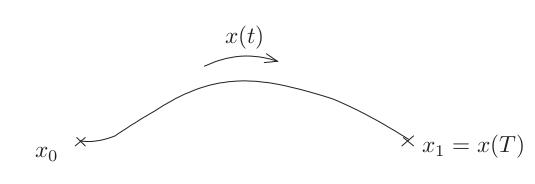
\includegraphics[width=\textwidth]{images/controle.png}
\end{figure}
Si la condition précédente est remplie, existe-t-il un contrôle joignant $\psi_0$ à $\psi_{cible}$ , et qui de plus minimise une certaine fonctionnelle $J(\varepsilon)$ ?
\subsection*{Contrôle optimal}
La fonctionnelle $J(\varepsilon)$ est un critère d’optimisation, on l’appelle le coût . Par exemple ce coût
peut être égal au temps de parcours; dans ce cas c’est le problème du temps minimal.
%Nous voulons construire un contrôle d'amplitude "raisonnable" afin d’amener le système d'un état initial $\psi_0$ à un état cible $O\psi(T)$. 
%$O$ étant l'observable décrivant l'état cible. \\\\
\begin{figure}[h]
	\caption{Problème de contrôle optimal}
	\centering
	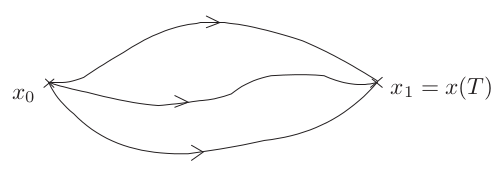
\includegraphics[width=\textwidth]{images/controleoptimal.png}
\end{figure}

On considère ainsi une fonctionnelle $J$
\begin{equation}
J(\varepsilon) = \langle \psi(T)|O|\psi(T) \rangle - \alpha \int_{0}^{T}\varepsilon^2(t)dt \quad \alpha \in \R_+
\end{equation}
et on se pose le problème: Trouver $\varepsilon$ tel que $\varepsilon$ résout
$$ \max_{\varepsilon \in L^2(0,T)} J(\varepsilon)$$
Au maximum de la fonctionnelle $J(\varepsilon)$, les équations de Euler-Lagrange sont satisfaites. Le Lagrangien du système est donné par :
\begin{equation} \label{lagrangien}
L(\psi,\varepsilon,\chi)= J(\varepsilon)\\
-2\Re \bigg\{ \int_{0}^{T}\langle \chi (t)|\partial_{t}+i(H_0+V-\mu(x)\varepsilon(t))|\psi(t) \rangle dt \bigg\}
\end{equation}
\section*{Schémas monotones}
Une stratégie éfficace de résolution de ces équations est donnée par une classe d’algorithmes relevant du contrôle quantique, les schémas monotones. Ils ont étés introduits en 1992 par David Tannor, Vladimir Kazakov et V. Orlov,  \cite{Tannor}, sur la base des travaux de Krotov \cite{Krotov1}, \cite{Krotov2}. Une amélioration a ensuite été proposée par Wusheng Zhu et Herschel Rabitz \cite{Zhu} en 1998. Une généralisation est donnée par Yvon Maday et Gabriel Turinici en 2003 \cite{Maday}.\\\\

Comment construire une discrétisation temporelle puis spaciale de ces algorithmes qui préserve la propriété de monotonie?\\\\

Dans le Chapitre Premier, nous introduisons la mécanique quantique en trois postulats et présentons le cadre général du contrôle quantique. Le Chapitre Deux est dédié aux schémas monotones pour l'équation de Schrödinger.
Différentes discrétisations de ces schémas sont proposées dans le Chapitre Trois.
\newpage
\chapter{Mécanique quantique et contrôle optimal}

\section{La mécanique quantique en trois postulats}
\subsection{Premier postulat de la mécanique quantique}
\subsubsection{Fonction d'onde}
Au mouvement de toute particule, on associe une fonction $\psi(x,t)$ appelée fonction d’onde. $\psi(x,t)$ nous donne toutes les informations sur l'état quantique de la particule a l’instant $t$.\\
\subsubsection{Cas d’une particule dans l’espace a une dimension}
(a mettre en subsssection)
A-Cas d’une particule dans l’espace a une dimension\\
La probabilité pour que la particule soit dans l’intervalle $[a,b]$ est donnée par l’aire de la courbe située entre $x=a$ et $x=b$ (figure si possible)
\begin{equation}
\int_a^b dP(x)= \int_a^b |\psi(x,t)|^2dx
\end{equation}
Il est impossible de connaître avec précision la position de la particule a un instant t. On ne peut que connaître la probabilité $dP(x)$ pour qu’elle soit entre $x$ et $x+dx$, soit:
\begin{equation}
dP(x)=|\psi(x,t)|^2dx=\psi(x,t)\overline{\psi(x,t)}dx
\end{equation}
La particule doit être quelque part sur l’axe $X’OX$, par conséquent:
\begin{equation}
\int_{-\infty}^{+\infty}|\psi(x,t)|^2dx=1
\end{equation}
pour tout $t$. $\psi$ est donc de carre sommable.
La densite de probabilite est donnee par
\begin{equation}
\frac{dP(x,t)}{dx}=|\psi(x,t)|^2=\rho(x,t)
\end{equation}

B-Cas d’une particule dans l’espace à trois dimensions\\
On a 
\begin{equation}
\int dP(\vec{r},t)=\iiint_{espace}|\psi(x,t)|^2d^3r=1
\end{equation}

Ou $d^3r$ représente l'élément de volume donnée par: $$d^3r=dxdydz=r^2sin\theta dr d\theta d\varphi$$

C-Cas de N particules\\
L’espace le mieux adapté à la description des systèmes en physique quantique est un espace $\Omega$, nommé espace des configurations qui représente l’ensemble de toutes les configurations possibles du système. Par exemple, dans le cas d’un système à $N$ particules isolées et sans contraintes, l’espace des configurations est $\Omega = \R^{3N}$ et $\psi(x,t) \in L^2(\Omega, \C)$.

\begin{Post}
	A tout système quantique correspond un espace de Hilbert complexe $\mathcal{H}$, tel que l’ensemble des états accessibles au système soit en bijection avec la sphère unité de $\mathcal{H}$.
\end{Post}
Dans la suite $\lVert\cdot\rVert$ et $\langle\cdot,\cdot\rangle$ désignent la norme et le produit hermitien associés à $\mathcal{H}$.
\subsubsection{Observables et deuxième postulat}
(talk about) Superposition des etats\\
(A beaucoup mieux traiter) (voir doc upmc)\\
En mécanique quantique, une grandeur ne prend une valeur déterminée que lors d’une mesure:
\begin{Post}
	A toute grandeur physique (scalaire) $\mathcal{A}$ correspond un opérateur $A$ auto-adjoint sur $\mathcal{H}$, vérifiant la propriété suivante : le résultat de la mesure d’une grandeur physique $\mathcal{A}$ ne peut être qu’un élément du spectre de $A$.
\end{Post}
La moyenne des mesures de $A$ est quant à elle égale à $\langle\psi|A|\psi\rangle$ où la notation $\langle\cdot|A|\cdot\rangle$ est définie par :
\begin{equation}
\langle\psi|A|\chi\rangle = \int_{\Omega} \bar{\psi}A\chi
\end{equation}
ou $\psi$ et $\chi$ sont des fonctions de $L^2(\Omega, \C)$ et $A$ un opérateur arbitraire défini de $L^2(\Omega, \C)$ dans lui-même.
(tableau observables)
\subsubsection{Equation de Schrödinger et troisième postulat}
L'équation de Schrodinger, conçue par le physicien autrichien Erwin Schrodinger en 1952, est une équation fondamentale en mécanique quantique. Elle décrit l'évolution dans le temps d’une particule massive non relativiste, et remplit ainsi le même rôle que la relation fondamentale de la dynamique en mécanique classique.
\begin{Post}
	Entre deux mesures, l’évolution de l’état est régie par l’équation de Schrödinger
	\begin{equation}
	i \frac{\partial }{\partial t} \psi (x,t) = H(x)\psi (x,t)
	\end{equation}
\end{Post}
%\input{chapitre2/}
%\input{chapitre3/}
%\chapter*{Conclusion et perspectives}\addcontentsline{toc}{chapter}{Conclusion et perspectives}

Le contrôle de l’équation de Schrödinger fait partie d’un domaine de recherche plus vaste appelé contrôle quantique. Le contrôle quantique a connu une activité intense ces deux dernières décennies; ce n'est pas surprenant compte tenu de l'importance de la modélisation quantique dans science des matériaux, conception de médicaments, biologie moléculaire, etc.\\
Dans ce mémoire, \\
Nous avons donc \\
Somme toute,\\

Dans un travail futur, nous pensons nous interesser à paralléliser sur plusieurs processeurs l'algorithme 
%\addcontentsline{toc}{chapter}{{Annexe}}
\lhead{\textsl{Annexe}}
\chapter*{Annexe}
\section*{Le logiciel Freefem++}
Voici un bref aperçu de ce logiciel.
Freefem++ [HP] est un logiciel libre de calcul scientifique, pour la résolution numérique d’équations aux dérivées partielles développé par Frédéric Hecht et Olivier Pironneau. Il est basé sur la méthode des éléments finis en dimension deux de l’espace. Il se caractérise par les principales fonctionnalités suivantes.
\begin{itemize}
\item La prise en compte sous forme variationnelle du problème à résoudre, qu’il soit linéaire, non linéaire, couplé, stationnaire ou évolutif en temps.
\item La génération automatique de maillages à partir d’une description simple (par morceaux) de sa frontière, y compris d’éventuels trous.
\item L’adaptation de maillage anisotrope basée sur une construction automatisée de métriques à partir de la matrice hessienne de fonctions freefem++.
\item Un large choix de types d’éléments finis : continus, discontinus, $P_k,1\leq k\leq3$ Lagrange, Raviart-Thomas... et de solveurs directs ou itératifs : (LU, Chosesky, Crout, Gradient Conjugué CG, GMRES, UMFPACK) avec des solveurs pour vecteurs propres et valeurs propres.
\end{itemize}
\section*{Programmes}
\begin{flushleft}
\textbf{Code Freefem++ pour la résolution du problème de Poisson.}
\end{flushleft}
\begin{figure}[!h]
\centering
\includegraphics[scale=0.9]{poissonCode2}
\end{figure}
\newpage
\textbf{Code Freefem++ avec adaptation de maillage pour la résolution du problème de Poisson.}
\begin{figure}[!h]
\centering
\includegraphics[scale=1]{poissonAdaptCode2}
\end{figure}
\newpage
\textbf{Ensemble des codes Scilab dans l'analyse de la méthode d'adaptation statistique en dimension 1.}
\begin{figure}[!h]
\centering
\includegraphics[scale=0.95]{CodesScilab1}
\end{figure}
\begin{figure}[!h]
\centering
\includegraphics[scale=0.99]{CodesScilab2}
\end{figure}
\begin{figure}[!h]
\centering
\includegraphics[ width =15cm , height =22cm ]{CodesScilab3}
\end{figure}
\[\]\[\]
\textbf{Ensemble des codes Feefem++ dans l'analyse de la méthode d'adaptation statistique en dimension 2}
\begin{figure}[!h]
\centering
\includegraphics[width =18.5cm , height =25cm ]{CodesFreefem++12}
\end{figure}
\begin{figure}[!h]
\centering
\includegraphics[width =18cm , height =25cm]{CodesFreefem++22}
\end{figure}
%\chapter*{{Bibliographie}}\addcontentsline{toc}{chapter}{{Bibliographie}}


\begin{thebibliography}{KNU90}\addcontentsline{toc}{chapter}{{Bibliographie}}
\bibitem{Krotov1} Krotov, V.F., Feldman, I.N.
\emph{Iterative methods for solving extreme problems}. In the
book: Modeling of technical and economic processes, Moscow, Moscow Economic and Statistical Institute (MESI) Publ. (1978), 54–65. (en russe)
\vspace{0.5cm}
\bibitem{Krotov2} Krotov, V.F., Feldman, I.N.
\emph{An iterative method for solving problems of optimal control}. Engineering Cybernetics, 21:2 (1983), 123–130.
\vspace{0.5cm}
\bibitem{Tannor} Tannor, D., Kazakov, V., Orlov, V.
\emph{Control of photochemical branching: Novel procedures for finding optimal pulses and global upper bounds}. Time Dependent Quantum Molecular Dynamics, edited by Broeckhove J. and Lathouwers L. Plenum, 347–360 (1992)
\vspace{0.5cm}
\bibitem{Zhu} Zhu, W., Rabitz, H.
\emph{A rapid monotonically convergent iteration algorithm for quantum optimal control over the expectation value of a positive definite operator}. J. Chem. Phys. 109, 385–391 (1998)
\vspace{0.5cm}
\bibitem{Maday} Maday, Y., Turinici, G. 
\emph{New formulations of monotonically convergent quantum control algorithms}. J. Chem. Phys. 118, 8191–8196 (2003)
\vspace{0.5cm}
\bibitem{Salomon} Maday, Y., Salomon, J. and Turinici, G..
\emph{Monotonic time-discretized schemes in quantum control}. Num. Math., 2005.
\vspace{0.5cm}
\bibitem{These} Salomon, J.
\emph{Contrôle en chimie quantique : conception et analyse de schémas d’optimisation}. 2005.
\vspace{0.5cm}
\bibitem{Strang} Strang, G. 
\emph{Accurate partial difference methods I: Linear Cauchy problems.}. Arch. Rat. Mech. and An. 12, 392–402 (1963)
\vspace{0.5cm}
\bibitem{Trelat} Trélat, E.
\emph{Contrôle optimal : théorie et applications}. avril 2016.
\vspace{0.5cm}
\bibitem{Fattorini} Fattorini, H.O., Kerber, A.
\emph{The Cauchy problem} Encyclopedia of mathematics and its applications 18. Section, Analysis. -Cambridge Press. 2009.
\vspace{0.5cm}
\bibitem{Dossa} Dossa, A.
\emph{Cours de Physique Quantique}. 2015-2016.
\vspace{0.5cm}
\bibitem{Glorieux} Glorieux, Q.
\emph{Cours 4 – Les principes de la mécanique quantique
3P001 – Universite Pierre et Marie Curie}. 2015-2016.
\vspace{0.5cm}
\bibitem{Dong} Dong, D., Petersen, I.R.
\emph{Quantum control theory and applications: A survey}. 2011.
\vspace{0.5cm}
\bibitem{Bidegaray} Bidégaray-Fesquet, B.
\emph{Méthodes numériques avancées pour la finance. — Méthodes de splitting}. 2009-2010.
\end{thebibliography}

%\bibliographystyle{plain}
%\bibliography{bibliographie}
\end{document}
